%!TEX root = ../dokumentation.tex

\chapter{Projekteinführung}
Die vorliegende Arbeit handelt von der Positionsbestimmung mittels Ultraschall, wie sie z.B. auch bereits für die Abstandsmessungen bei PKWs (Einparkhilfen) eingesetzt wird. Dabei gibt es zwei unterschiedliche Methoden, um die Abstände zwischen zwei oder mehr Gegenständen zu ermitteln. Entweder führt man eine direkte oder eine indirekte Messung durch. Für eine direkte Messung ist es nötig, dass die Position zweier Punkte, deren Abstand man messen möchte, bekannt ist. Dann wird eine unmittelbare Abstandsmessung mit Hilfe eines Maßstabes (z.B. Zentimeter) durchgeführt, um den Abstand zwischen den beiden Punkten zu bestimmen. Um allerdings unabhängig von der Position den Abstand ermitteln zu können, bedarf es einer indirekten Abstandsmessung. Diese erfolgt indem nicht die Entfernung direkt, sondern eine von ihr abhängige Größe ( die Signallaufzeit) gemessen wird. Im Folgenden Versuchsaufbau soll die Position eines Gegenstands ermittelt werden, welcher sich im Wellenkegel dreier Ultraschallsender bzw. Empfänger befindet. Bevor jedoch die eigentliche Messung gestartet wird, ermittelt man zunächst die relative Position der Sender-Empfänger-Konstruktionen im Raum, indem einer der Sender ein Ultraschallsignal aussendet, welches von den Empfängern der  jeweils anderen Sender-Empfänger-Konstruktionen empfangen wird. Über die bereits erwähnte Signallaufzeit, lässt sich der Abstand zwischen den beiden Sender-Empfänger-Konstruktionen messen. Mittels Trilateration kann so die genaue Position der drei Sender-Empfänger-Konstruktionen ermittelt werden. Nach dem selben Prinzip wird dann letzten Endes auch die Position und der Abstand zum Gegenstand in deren Mitte bestimmt.\\
Die vorliegende Arbeit enthält die theoretischen Grundlagen, die notwendigen Konstruktionsanleitungen der entwickelten und genutzten Bauteile, sowie die Beschreibung der Oberfläche für die Darstellung der Messergebnisse. Außerdem noch die wichtigsten Problembehandlungen, sowie die notwendige Schnittstellenkommunikation.


\section{Ultraschall Grundlagen}
Bevor der genaue Vorgang bei der Positionsbestimmung mittels Ultraschalls beschrieben wird, sollen hier zunächst einige Grundlagen und Kenntnisse über den Ultraschall im Allgemeinen zum besseren Verständnis beitragen:
\subsection{Was genau ist Ultraschall?}
Bei Ultraschall handelt es sich um Schallfrequenzen, oberhalb des hörbaren Frequenzbereichs des Menschen. Diese Aussage zu präzisieren ist allerdings schwierig, denn dieser Bereich unterliegt individuellen Wahrnehmungsschwankungen und um-fasst daher Frequenzen ab etwa 16 kHz.\footnote{nach DIN 1320 Akustik Begriffe} Bei Frequenzen unterhalb des für Menschen hörbaren Bereichs handelt es sich um Infraschall. Ab einer Schallfrequenz von etwa $1GHz$ spricht man von Hyperschall. 
\begin{figure}[H]
	\centering
	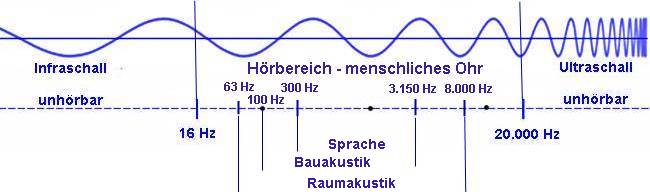
\includegraphics[scale=0.9]{images/hoerbarer_Schall-Infraschall-Ultraschall.jpg}
	\caption{Frequenzbereich des Schalls\footnotemark}
\end{figure}
\footnotetext{\url{http://www.haustechnikdialog.de/SHKwissen/Images/hoerbarer\_Schall-Infraschall-Ultraschall.jpg}}


\subsection{Wie breitet sich Ultraschall aus?}
Die Ausbreitung der Ultraschallwellen hängt von der Beschaffenheit des zu durch-dringenden Mediums ab: Im Innern von Gasen und Flüssigkeiten breitet sich Ultraschall überwiegend als Longitudinalwelle (Längswellen - Schwingungsrichtung der einzelnen Oszillatoren ist parallel zur Ausbreitungsrichtung der Welle) aus. In Festkörpern kommt es jedoch zu Schubspannungen die dazu führen, dass die Ultraschallwellen sich zusätzlich in Transversalwellen (Schwingungsrichtung der einzelnen Oszillatoren ist orthogonal zur Ausbreitungsrichtung der Welle) ausbreiten.
Prinzipiell erfährt die Schallwelle bei der Ausbreitung einen Verlust an Schallintensität und der damit verbundenen Schallfeldgrößen. Diese werden beim Durchdringen eines Mediums durch Absorption, Reflexion, Brechung, Streuung und Schallfeldgeometrie abgeschwächt. Ursachen für die Absorption sind: innere Reibung, Wärmeleitung und Relaxationen. Die Absorption führt dazu, dass die Schallwellenreichweite begrenzt ist und die Frequenz an die Eindringtiefe angepasst werden muss. Luft weist eine stark mit der Frequenz steigende Dämpfung für Ultraschall auf, was für den späteren Versuchsaufbau dieser Arbeit von Bedeutung sein wird. \\
Der Zusammenhang zwischen der Frequenz $\nu $ und der Wellenlänge $\lambda$ der Schallwelle ist formal derselbe wie beim Licht, allerdings mit anderer Ausbreitungsgeschwindigkeit fehlender Dispersion:
\begin{equation}
c=\lambda*\nu
\end{equation}
Weil es sich bei Schallwellen um longitudinale Materie-Wellen handelt können diese sich auch nicht in einem Vakuum ausbreiten (physikalisch gesehen ist Schall eine als Welle fortschreitende mechanische Deformation in einem Medium und braucht daher immer ein Trägermedium, z.B. Luft). 


\section{Indirekte Abstandsmessung durch Laufzeitmessung}
Das Prinzip, welches hinter einer Abstandsbestimmung mittels Laufzeitmessung steckt, entspricht dem eines Echos. Wegen der zugrundeliegenden, physikalischen Eigenschaft mancher Materialien den Schall zu reflektieren kann daraus eine Methode zur Abstandsbestimmung abgeleitet werden. Ein Schallimpuls (Rufen) wird losgeschickt, am Hindernis reflektiert und die Zeit bis zu seiner Rückkehr (Echo) zur Schallquelle gemessen. Anhand der bekannten Ausbreitungsgeschwindigkeit des Schalls in Luft lässt sich die Entfernung zum Hindernis berechnen.


\begin{figure}[H]
	\centering
	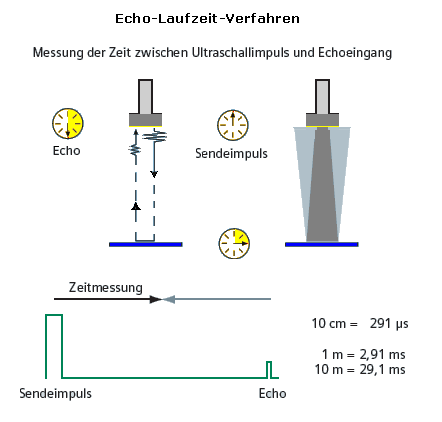
\includegraphics[scale=0.8]{images/Echo-Laufzeit-Verfahren.png}
	\caption{Echo-Laufzeit-Verfahren\footnotemark}
\end{figure}
\footnotetext{\url{https://de.wikipedia.org/wiki/Ultraschall}}

Bei Laufzeitmessungen werden im Wesentlichen nur Zeitdifferenzen bestimmt. Daher benötigt man- im Gegensatz zu Messungen in einer absoluten Zeitskala (Weltzeit, Atomzeit usw.)- nur ein relatives Zeitsystem, also ohne definierten Nullpunkt.

\subsection{Das Echosignal}
Ein Echosignal setzt sich aus verschiedenen Signalanteilen zusammen:
\begin{figure}[H]
	\centering
	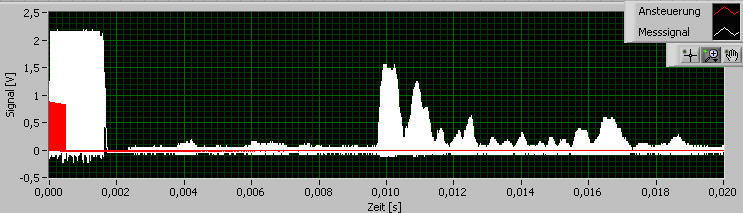
\includegraphics[scale=0.6]{images/echosignal.png}
	\caption{Aufnahme eines Echosignals\footnotemark}
\end{figure}
\footnotetext{\url{http://tu-dresden.de/die\_tu\_dresden/fakultaeten/fakultaet\_elektrotechnik\_und\_informationstechnik/iee/mst/studium/lehre/MST/dl/Pr/us}}

Ganz vorne links ist der gesendete Ultraschallimpuls zu sehen. Dieser Puls ist bereits auffallend länger als das tatsächliche Ansteuersignal. Der Grund hierfür ist das lange Ausschwingen des Ultraschallwandlers und die Verstärkerelektronik. Infolge dessen kann es zu einer Überlagerung des ausschwingenden Sendepulses mit dem ersten Echosignal kommen was wiederum zu einer Begrenzung des minimal messbaren Abstands führt.\\
Weiter rechts in der Abbildung sind die eigentlichen Reflexionen des Ultraschallpulses zu sehen, gefolgt von weiteren Überlagerungen, die durch unmittelbare Reflexion des Hindernisses als auch aus Mehrfachreflexionen bestehen. Diese Mehrfachreflexion ist die fortlaufende Reflexion eines früheren Ultraschallpulses zwischen dem Hindernis und der Messvorichtung. Dieser Hin- und herlaufende Ultraschallpuls wird zwar zunehmend gedämpft, wird jedoch trotzdem mit kleinerer Amplitude in den nachfolgenden Echosignalen sichtbar bleiben.\\
Das Auftreten dieser Mehrfachreflexionen führt zu einem komplexen Aussehen des zu deutenden Echosignals und erschwert die Erkennung des eigentlichen Echos des Hindernisses. Daher muss die Erkennung mit Hilfe eines Schwellwertes erfolgen, welcher jedoch für eine begrenzte Verlässlichkeit der Abstandsmessung sorgt.

\subsection{Ultraschallsender}
Um Ultraschall zu erzeugen eignen sich dynamische und elektrostatische Lautsprecher, sowie insbesondere Piezolautsprecher.  Bei letzterem handelt es sich um Membran-gekoppelte Platten aus piezoelektrischer Keramik, die durch Umkehr des Piezo-Effekts\footnote{Änderung der elektrischen Polarisation und somit das Auftreten einer elektrischen Spannung an Festkörpern, wenn sie elastisch verformt werden} zu Schwingungen angeregt werden. Mit Hilfe von piezoelektrischer Kunststoffe (PVDF) lassen sich auch direkt Membranen ansteuern, was ein verbessertes Übertragungsverhalten hervorruft.

\subsection{Ultraschallempfänger}
Der Empfang von Ultraschallwellen kann prinzipiell mit den gleichen elektrischen Wandlern erfolgen, wie sie auch zu dessen Erzeugung verwendet werden. Die so erhaltenen elektrischen Signale können einer Frequenz-, Phasen- oder Amplitudenauswertung unterzogen werden.

\section{Positionsbestimmung}
Für die Positionsbestimmung eines Gegenstands, welcher sich zwischen drei Ultraschallsensoren befindet muss zunächst die genaue Position der Sensoren festgelegt, bzw. ermittelt werden. Dies erfolgt ebenfalls über eine Abstandsmessung: 
Abwechselnd senden die Sender einen Ultraschallimpuls, und ermitteln mittels eines direkt daneben angebrachten Empfängers den Abstand zum nächsten Sensor. Da nicht alle Sensoren exakt gleich gut messen werden die beiden Abstandswerte zwischen zwei Sensoren im Anschluss noch gemittelt. Direkt danach messen die Sensoren den Abstand zum Gegenstand in der Mitte bestimmen dadurch dessen genaue Position.

